\chapter{Structured Prediction}\label{sec:ml}

In this section we lay out the basic definitions and tools necessary for 
data-driven modeling of {\em classification problems}.  In the most general 
setting, the goal is to learn a mapping, or {\em classifier}, $h$ in a 
hypothesis class $\cH$ from a set of input examples $x$ to a set of discrete 
output variables $y$.   We concern ourselves in this work with a specific 
setting: $x$ lies in a (possibly high-dimensional) vector space (most commonly 
in this work, the input image pixels) and the target lies in a discrete 
$n$-dimensional space: $$y \in \{0,1,\ldots,k\}^n \defn \cY.$$  

We will refer to the set $\cY = \{0,1,\ldots,k\}^n$ as the set of labels, {\em 
label set}, or {\em state space} for a dimension of $y$.  The $i^{th}$ 
dimension of $y$ will be indexed $y_i$, and referred to as {\em variable} $i$.  
We refer to the state space of part $i$ as $\cY_i$, and the size of the state 
space as $|\cY_i|$.  The size of the full state space is $|\cY| = |\cY_1 \times 
\ldots \times \cY_n|$, where here $\times$ denotes a Cartesian product.

For example, in a simple image classification task to determine whether an 
image has a dog in it, $x$ could be an image's pixels, and $y \in \{dog, 
not~dog\} \cong \{0,1\} $; an instance of {\em binary classification}.  In this 
case, $k = 2$ and $n = 1$.  In {\em multiclass classification}, $k>2$ and $n = 
1$, \eg, predicting the handwritten digits $0,\dots,9$ or the weather $\{sunny, 
cloudy, rainy\} \cong \{0,1,2\}$.  Finally, in {\em structured prediction}, the 
output $y$ is a vector: $n > 1$.

We will discuss four major components necessary for learning and applying 
machine learning classifiers in this chapter:

\begin{itemize}
\item An {\bf inference procedure} to determine the most likely label for a 
fixed test example $x$: \begin{equation}
h(x) \triangleq \argmax_{y \in \cY} h(x,y).
\end{equation}
\item The {\bf hypothesis class $\cH$} from which to obtain our classifier $h$.
\item  A {\bf learning loss function} $\cL(\cdot)$ which assesses the quality 
of any particular classifier $h \in \cH$.
\item A {\bf learning algorithm} to find the minimizer of $\cL$: 
\begin{equation}
h = \argmin_{h' \in \cH} \cL(h').
\end{equation}
\end{itemize}

\out{
\begin{table}[tb!]
\centering
\begin{tabular}{| c | c | }
\hline
symbol & definition \\
\hline
\hline
$x \in \cX = \reals^d$ & input variables\\
$y \in \cY =\{0,1,\ldots,k\}^n$ & output variables \\
$h(x,y): \cX \times \cY \mapsto \cY$ & classifier \\
\hline
\end{tabular}
\caption[Machine learning notation]{Machine learning notation.}
\label{tab:notation}
\end{table}
}


\section{Generalized linear classifiers}\label{sec:glms}
There are many possible parametric and non-parametric choices of hypothesis 
classes $\cH$ to consider.  One of the easiest to represent, learn, visualize 
and analyze is the hypothesis class of {\em generalized linear models}, of the 
form
\begin{equation}
h(x,y) = \sum_{i=1}^d w_i f_i(x,y)\ = \w \cdot \f(x,y) \end{equation}
where $\w \in \reals^d$ is a vector of linear parameters of our model and 
$\f(x,y) \in \reals^d$ is a vector of features that depend on the input and 
output variables.  Thus the model is simply a weighted sum of features to 
obtain a real-valued score, and $\cH = \reals^d$.


\begin{figure}[tb]
\begin{center}
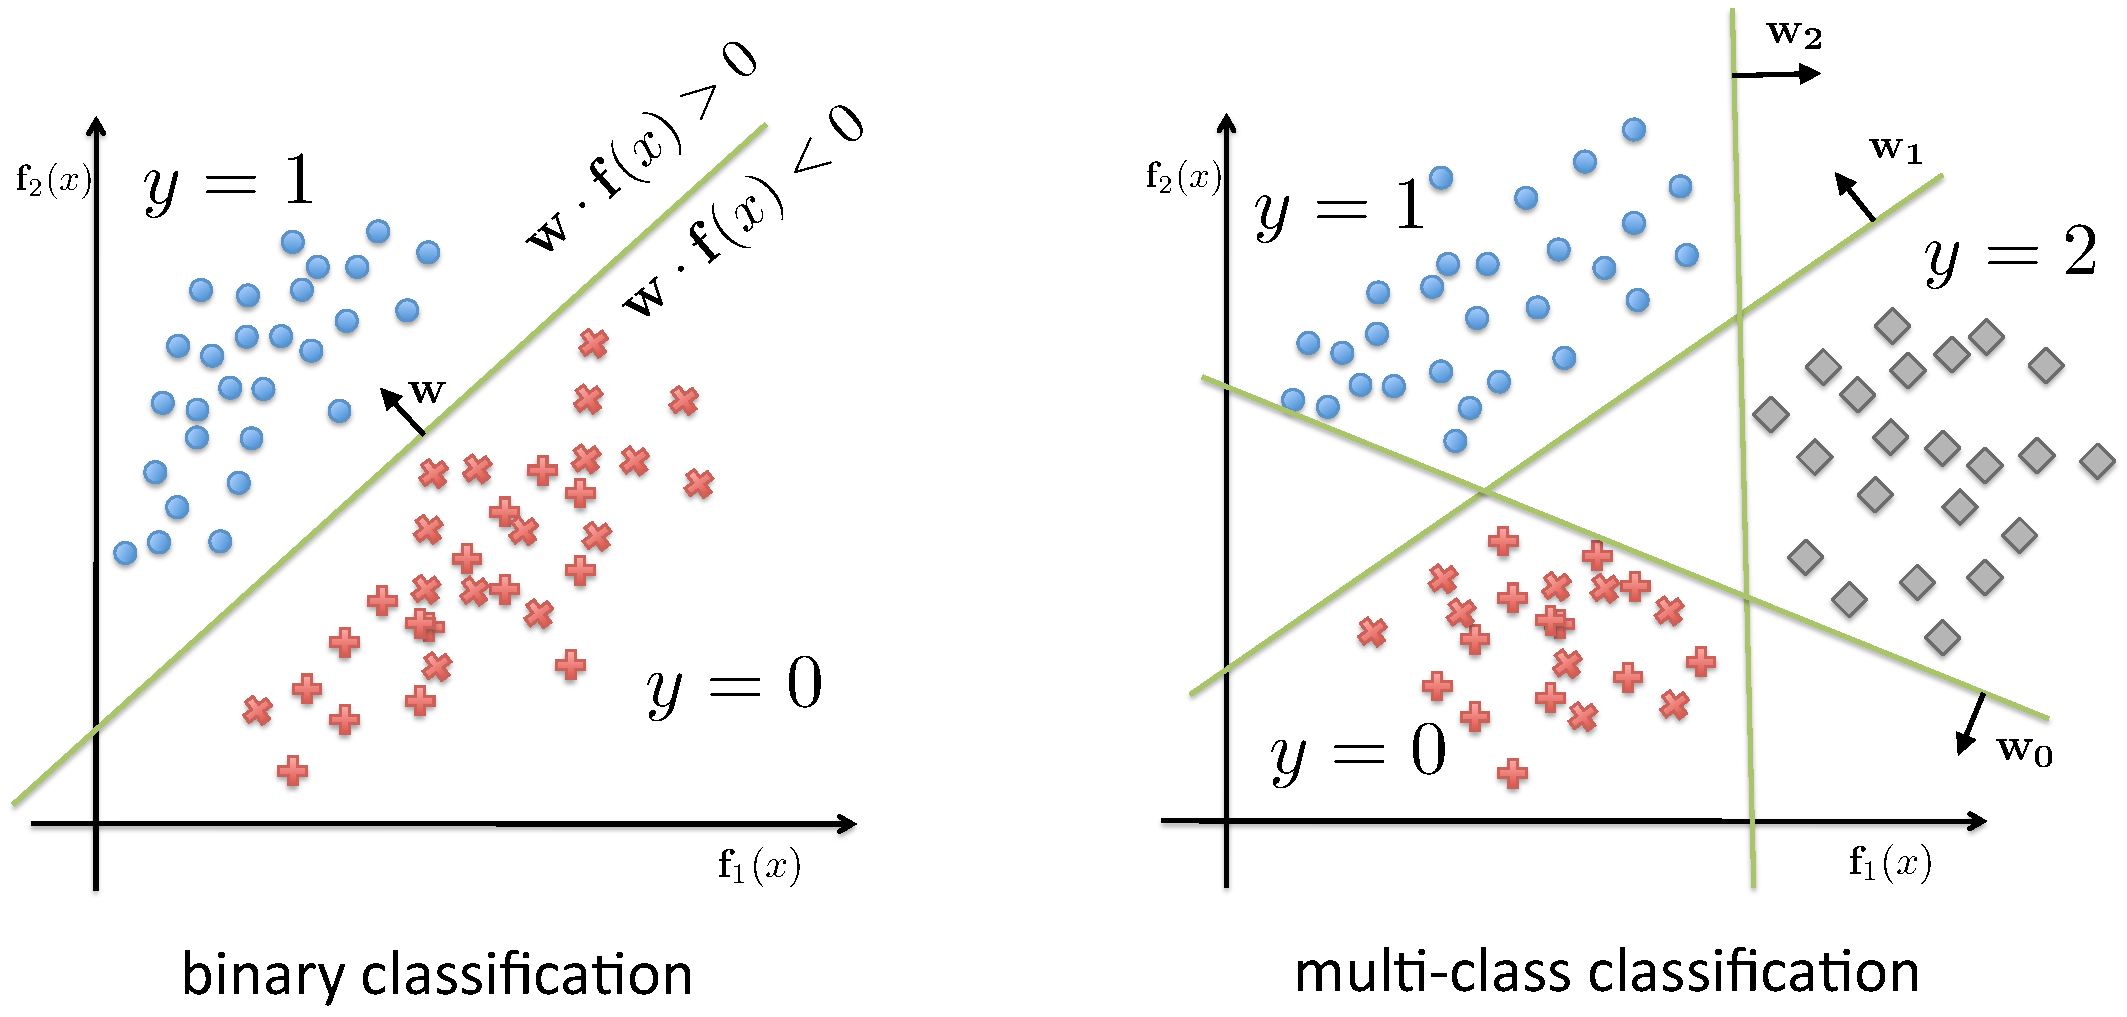
\includegraphics[width=0.95\textwidth]{figs/binary-multiclass-ml.pdf}
\caption[Binary and multi-class linear classification.]{Binary and multi-class classification.  On the left is shown a binary labeling problem in 2 dimensions, with a linear classifier which perfectly classifies the data.  On the right is shown a 3 class classification problem, with a linear classifier for each class, each of which perfectly separates the correct label from the two incorrect labels.}
\label{fig:binary-multiclass-ml}
\end{center}
\end{figure}


\subsection{Binary and multi-class classifiers}
\label{sec:binary-multi-class}
In binary ($y \in \{0,1\}$) and multi-class ($y \in \{0,\ldots,k\}$) 
classification problems, there is a simple and intuitive geometric 
interpretation to linear classifiers.  In two dimensions, the classifiers 
describe a line, in three dimensions, they describe a plane, and in general, 
they describe a {\em hyperplane} which partitions the feature space (for a 
particular label) into two halfspaces.  

Observe that for binary classification, we need only look at which side of a 
hyperplane a point lies on in a particular feature space to determine the 
label:
\begin{align}
h(x) &= \Ind\left( h(x,1) > h(x,0)\right) \\
&= \Ind\left( \w \cdot \f(x,1) > \w \cdot \f(x,0) \right) \\
&= \w \cdot \left(f(x,1) - f(x,0)\right)  > 0\\ 
&= \w \cdot \tilde{f}(x) > 0 
\end{align}

The vector $\w$ describes a hyperplane via its surface normal.  The test $\w 
\cdot \tilde{f}(x) > 0$ determines which side of the hyperplane an example lies 
on, which also corresponds to its predicted label, as 
in \figreff{binary-multiclass-ml}{left}.  When $k > 2$, we can also transform 
feature spaces and interpret the linear classifier as $k$ separating 
hyperplanes in $d$ dimensions, one hyperplane to separate each label from the 
rest.  \figreff{binary-multiclass-ml}{right} illustrates an example with $k = 
3$ and $d = 2$.

\section{Pairwise structured models}
\label{sec:mrfs}
In structured prediction, the output space $|\cY| = |\{0,\ldots,k\}^n|$ is 
exponential in $n$ and typically enormous. Due to computational and modeling 
considerations to be discussed, we assume that the full model $\w \cdot 
\f(x,y)$ {\em decomposes} into {\em factors}, or {\em cliques} which involve 
overlapping sets of variables:  \begin{equation}
\w \cdot \f(x,y) = \sum_{c \in \cC} \w_c \cdot \f_c(x,y_c) = \sum_{c \in \cC} 
\phi_c(x,y_c),
\end{equation}
where we use the shorthand for factors $\phi_c(\cdot) \defn \w_c \cdot 
\f(\cdot)$.  The index $c$ represents a set of components of $y$ and $\f$, \eg, 
$y_c = \{y_1,y_2,y_3\}$. The set $\cC$ is the set of all factors $c$ in our 
model.  We can encode the sets of factors and their overlap relations in 
general using a {\em factor graph} \citep{koller-book}.  The number of 
different settings and representations for structured models is vast and varied 
and most are outside the scope of this work.  

For our purposes, we focus on structured problems with at most {\em pairwise 
structure}, where $|c| \leq 2\;\; \forall c \in \cC$\footnote{This 
simplification does not result in loss of generality, as factors involving 3 or 
more variables can always be converted into pairwise or unary factors with an 
expanded label set consisting of the Cartesian product of each variable's state 
space. For example, a factor involving the variables $y_1,y_2$ and $y_3$ with 
state space $\{1,\ldots,k\}^3$ can be converted into a single variable $y_{123} 
\in \{1,\ldots,k^3\}$.  This transformation is, however, exponential in 
$|c|$.}.  We can represent a pairwise structured model as a graph $G = 
(\cV_G,\cE_G)$ where each variable $y_i$ corresponds to a vertex in the graph's 
vertex set $\cV_G$, and each edge in $\cE_G$ corresponds to two variables 
$y_i,y_j$ being involved in a pairwise factor $\phi_{ij}$.  We can then 
decompose our classifier into the special form
\begin{align}
\w \cdot \f(x,y) &= \sum_{i \in \cV_G} \w_i \cdot \f(x,y_i) + \sum_{i,j \in 
\cE_G} \w_{ij} \cdot \f(x,y_i,y_j) \\
& = \sum_{i \in \cV_G} \phi_i + \sum_{i,j \in \cE_G} \phi_{ij}.
\label{eq:mrf}
\end{align} There is a huge amount of research dedicated to models of this form 
originally stemming from statistical mechanics, where it was first used to 
determine the spin of particles arranged in a grid. From this perspective, 
\equref{mrf} describes the log of the energy of the particle system.  When 
given a probabilistic interpretation (as we will see in \secref{probinterp})
this type of model is known as a {\em pairwise Markov Random Field} (MRF).  
Because of such historical intuitions as a model for energy, we refer to the 
different terms as {\em potentials}, and \equref{mrf} as the negative of an 
{\em energy function} which we seek to minimize.  Terms of the form $\phi_i = 
\w_i \cdot \f_i$ we will refer to as {\em unary potentials}; $\phi_{ij} = 
\w_{ij} \cdot \f_{ij}$ are {\em pairwise potentials}.

\subsubsection{Pairwise MRF examples}\label{sec:pairwise-mrf}
\begin{figure}[tb]
\begin{center}
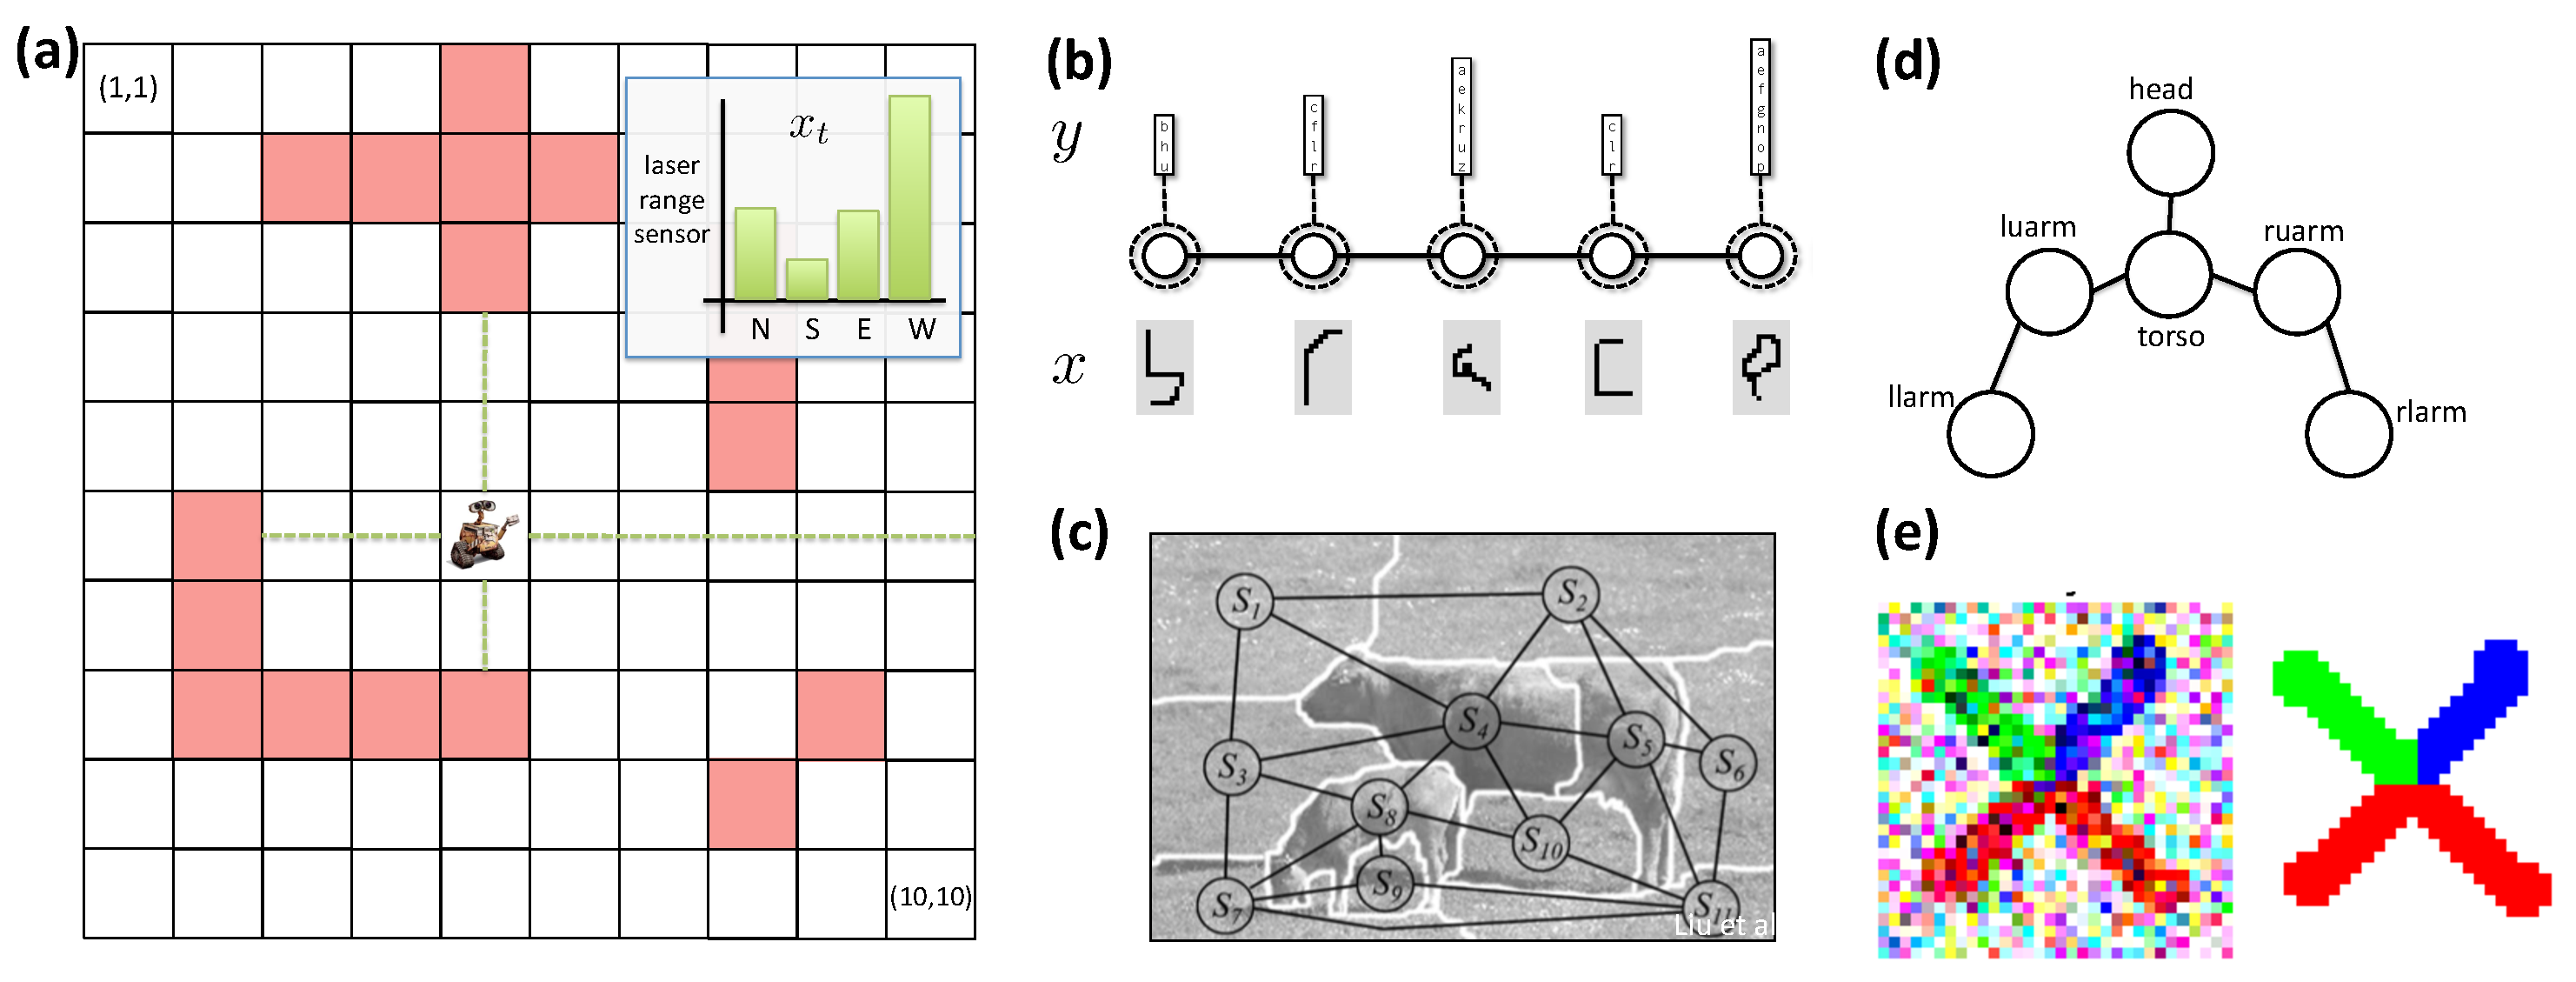
\includegraphics[width=0.95\textwidth]{figs/mrf-examples.pdf}
\caption[MRF examples]{MRF examples.  (a) A robot localization problem on a $10 
\times 10$ grid. (b) Handwriting recognition.  (c) Scene labeling.  (d) Human 
pose estimation.  (e) Image denoising. See text for details. }
\label{fig:mrf-examples}
\end{center}
\end{figure}



Our primary application of interest in this work is human pose estimation, 
whose modeling as an MRF will be discussed in detail in \secref{ps}.  However, 
to first give motivation and intuition about how and why to model problems via 
a pairwise MRF, we present a few vision- and robotics-related examples here.

\mypar{Wandering robot}
Imagine we are tracking the location of a robot on a map with 100 locations 
over 100 time steps as in \figreff{mrf-examples}{a}.  We have no idea what the 
robot's intent is or where he starts out in the world (the ``kidnapped robot'' 
scenario), only that he is restricted to moving adjacent grid positions at each 
time step (\ie, cannot teleport).  We have noisy sensor readings $x = 
[x_1,\ldots,x_{100}]$ for every time step.  The output $y$ is a sequence of 
locations the robot visited in all 100 time steps, one out of $\cY = 100^{100} 
= 10^{1000}$ possibilities.  By comparison, the estimated number of atoms in 
the universe is only $10^{80}$.  A \naive approach would be to model this as a 
multi-class problem with $10^{1000}$ labels, and try to directly learn a 
mapping $h(x,y) = \w \cdot \f(x,y)$ for all possible $y$.  Importantly, there 
is a lot of {\em structure} to this problem, the most obvious being that many 
outputs $y$ are just not valid, due to the fact that the robot can only move to 
an adjacent location at each step.

The key insight to be made is the following: knowing where the robot is at time 
$t$ is tremendously useful for determining the robot's next location at 
$t+1$---the robot must be somewhere in the vicinity.  In addition, knowing 
where the robot is at $t-1$ also helps localize it at $t+1$, but with 
diminishing returns---we now know its previous velocity.  Going further into 
the past, there is increasingly less information to help localize where the 
robot is at time $t+1$.
In general, we can make the simplifying assumption that {\em given the recent 
past, the future is independent of the distant past}.  Using this intuition, we 
can model the problem as a {\em chain} MRF:
\begin{equation}
\w \cdot \f(x,y) = \sum_{t=1}^{100} \phi_t(x,y_t) + \sum_{t=1}^{99} 
\phi_{t,t+1}(y_t,y_{t+1})
\end{equation}
where the graph structure is a node for the output variable at each time step 
$y_t$, and we only consider pairwise factors over adjacent time steps 
$\phi_{t,t+1}$, creating a chain of variable interactions.  The unary 
potentials $\phi_t$ can model the likelihood of being in each grid location at 
time $t$ based on sensor readings, and the pairwise potentials can model how 
likely it is to transition from any location $y_t$ to any location $y_{t+1}$.  

The pairwise term in such tracking problems is typically represented as a {\em 
transition matrix}.  In this robot localization problem the transition matrix 
would be very sparse, since any location can only transition to adjacent grid 
locations.  It might be comprised of the values $\{-\infty,0\}$ indicating 
which transitions are or aren't possible, or more generally, log-probabilities 
of how likely different transitions are: $\phi_{t,t+1}(y_t,y_{t+1}) \propto 
\log p(y_{t+1} | y_t)$.


In other structured problems, it also makes sense to make {\em independence 
assumptions} about which dimensions of $y$ are assumed dependent on each other 
and their interactions should be directly modeled. For example: 

\mypar{Handwriting recognition} In this problem, the output at each position is 
which letter of the alphabet is written given handdrawn letter images $x$ (in 
this problem, $k=26$ if only considering `a',\ldots,`z', or roughly $70$ if 
considering all alphanumerics plus punctuation).  Clearly adjacent letters in a 
document are highly correlated (\eg, adjacent outputs such as `ab' and `he' are 
likely, but `hb' is not), but depend very little on letters far away in the 
word, sentence or even document.  Practitioners again typically model this as a 
chain, seen \figreff{mrf-examples}{b}.

\mypar{Scene labeling} In scene labeling, the goal is to label coarse segments 
of an image with scene types (``sky'',``grass'',``building'',``cow'', etcetera; 
$k$ is on the order of tens of labels) given the image as $x$. The typical 
assumption made is that adjacent regions' labels directly depend on each other, 
whereas the label of spatially distant segments have weak or no interactions 
and are not modeled \citep{cour05}.  The MRF model thus connects adjacent 
segments in the image, giving us a cyclic planar graph as in
\figreff{mrf-examples}{c}.

\mypar{Human pose estimation}  Knowing the location of the left shoulder is a 
strong cue for where the left elbow should be, since they are kinematically 
coupled in the real world, but only a weak indicator of where the right wrist 
should be.  The typical representation is to describe the human layout as a 
tree graph corresponding to the kinematic skeleton, see 
\figreff{mrf-examples}{d} and \secref{ps}.


\mypar{Image denoising} Here the input $x$ is an image with a small set of 
labels that are corrupted by noise; the goal is to determine the uncorrupted 
original image $y$ the same size as $x$.  In this setting $k$ is typically 2 or 
a small set of indexed colors. Practitioners typically model this problem with 
a grid graph, where variable $y_{(r,c)}$ corresponds to pixel label at row $r$, 
column $c$, and is in pairwise factors with 
$y_{(r+1,c)},~y_{(r-1,c)},~y_{(r,c+1)}, \text{ and } y_{(r,c-1)}$.  Pairwise 
terms model the assumption that adjacent pixels are likely to have the same 
label, \eg, $\phi_{(r,c),(r+1,c)} \propto \ind{y_{(r,c)} = y_{(r+1,c)}}$.  See 
\figreff{mrf-examples}{e}.

You may object that some of the decomposition assumptions made in the above 
examples are somewhat extreme.  However, they are typically seen as forgivable 
thanks to the greater simplicity of modeling only local interactions. Even more 
enticing is the reduction in computation they allow, discussed in 
\secref{inference}.

\subsection{Probabilistic interpretation}\label{sec:probinterp}
Much of the development of machine learning models and methods originally came 
from the probabilistic modeling and statistics literature 
\citep{koller-book,esl-book,bishop-book}.  From this perspective, our model 
describes a {\em log-linear} probabilistic form of the posterior probability 
$p(y|x)$:
\begin{equation}
p(y|x)= \frac{\exp \left[ \w \cdot \f(x,y) \right]}{\sum_{y \in \cY} \exp \left[\w \cdot f(x,y) \right]} = \frac{1}{Z(x)} \exp \left[ \w \cdot \f(x,y) \right]
\end{equation}
It can be shown that this particular form of $p(y|x)$ is the
distribution with maximum entropy, subject to the constraints that feature 
expectations with respect to $p(y|x)$ match empirical feature expectations in a 
training set \citep{jaynes1963}.  This principle is based on the desire to have 
our model make as few assumptions as possible (be most entropic) about the 
observed data.

Because we are typically only interested in the most likely $y$---here, the 
{\em maximum a posteriori} or MAP assignment---it is sufficient to find the 
$\argmax$ of a simplified quantity and not worry about normalization by $Z(x)$:

\begin{align}
&\argmax_y p(y|x) \\
&= \argmax_y \log p(y|x) \\
&= \argmax_y \w \cdot \f(x,y) - \log Z(x) \\
&= \argmax \w \cdot \f(x,y)
\end{align}

A distribution $p(y|x)$ modeling a structured $y$ that decomposes over factors 
as in \secref{pairwise-mrf} takes the form:
\begin{equation}
p(y|x) \propto\exp\left[  \sum_{i \in \cV_G} \phi_i + \sum_{i,j \in \cE_G}  
\phi_{ij}\right] = \prod_{i \in \cV_G} \exp \phi_i  \prod_{i,j \in \cE_G} \exp 
\phi_{ij}
\label{eq:crf}
\end{equation}
Historically and in other settings, terms $\exp \phi_c$ were assumed to be 
themselves proper joint $p(y_c,x)$ or posterior $p(y_c|x)$ distributions over 
subsets of random variables $c$, but we assume no such restriction in our case.  

Sometimes people make distinctions between fitting parameters for a {\em 
generative model} of the form $p(x,y)$ versus a {\em discriminative model} of 
the form by referring to the former as a Markov Random Field, and the latter as 
a {\em Conditional Random Field} (CRF) \citep{lafferty01crfs} or {\em 
Discriminative Random Field} \citep{kumar2003discriminative}.  The differences 
between MRFs and CRFs lie in the way in which models of the form~\equref{crf} 
are trained, and restrictions on the form of the potentials allowed.  

In all our work, we assume no restrictions on the form of potentials, always 
assume $x$ is given and $y$ is to be estimated, and learn a discriminative 
model, like a CRF (see \secref{learning}).  However, we never use a 
probabilistic interpretation of our model nor compute the distribution 
normalizing constant.  We prefer to use the generic term MRF for the rest of 
the paper, under the view that all these models are simply general linear 
models in a high dimensional space, with decomposable structure.  At test time, 
the inference algorithms are the same.  

\section{Inference}
\label{sec:inference}
The inference problem is to determine the highest scoring possibility out of 
all possible outputs in $\cY$: 
\begin{equation} 
y^\star = h(x) = \argmax_{y \in \cY} h(x,y).  
\end{equation}
We use the convention $h$ to mean {\em hypothesis} or {\em hypothesis class}, originating from the machine learning community.  In the spirit of optimization, we also view this as a {\em scoring function} and use the synonymous notation $s$ to denote the score:
\begin{align} s(x,y) &\defn h(x,y) \end{align}
When $\cY$ is low-dimensional, brute-force search is easy enough: evaluate 
$s(x,y)$ for all possible $y$, and return the highest scoring.  This is 
possible for both binary and multi-class classification, where we evaluate up 
to $k$ possible labels to determine the highest scoring.

However, in the most general setting, the size of $\cY$ is exponential in $k$: 
$|\cY| = k^n$, and we can't hope to enumerate all possible outputs in $\cY$ to 
find the highest-scoring.  Thankfully, the decomposable structure we impose on 
our models, discussed in \secref{mrfs}, allows us to find a solution time 
polynomial in $k$ and linear in $n$.
 

As a simple example of this, consider our wandering robot problem 
(\secref{pairwise-mrf}) where we make the common assumption that we only model 
temporally adjacent pairs of output variables together, making a chain of 
variable dependencies:
\begin{equation*}
\w \cdot \f(x,y) = \sum_{t=1}^{100} \phi_t(x,y_t) + \sum_{t=1}^{99} 
\phi_{t,t+1}(x,y_t,y_{t+1})
\end{equation*}
Observe now how computing the maximum score of the classifier {\em also 
decomposes} for this simple problem:
\begin{align}
&\max_{y \in \cY} \w \cdot \f(x,y) = \max_{y_1,\ldots,y_{100}} 
\sum_{t=1}^{100} \phi_t(x,y_t) + \sum_{t=1}^{99} \phi_{t,t+1}(x,y_t,y_{t+1}) \\
&= \max_{y_{100}} \left[ \phi_{99,100} + \phi_{100} + \ldots \max_{y_3} \left[\phi_{3,4} + \phi_3 +  \max_{y_2} \left[ \phi_{2,3} + \phi_2 + \max_{y_1} \phi_{1,2} + \phi_1 \right] \right] \ldots \right] 
\label{eq:nesting} \end{align} 
In \equref{nesting}, we see that the max over each dimension of $y$ can be
nested and needs only reason over at largest a pairwise factor at a time.  In 
our robot problem, each pairwise factor is only $100^2$ numbers to consider and 
each unary factor is of size $100$. Thus the total amount of numbers that need 
to be examined in this problem is roughly $10^6$, an astronomical improvement 
over the complete space of $10^{1000}$. In general the bottleneck of inference 
is the max over the pairwise factors having size $k^2$, and thus inference is 
$O(n \cdot k^2)$.

When an MRF model forms a tree, we can always exploit the structure in a 
similar way for exact efficient inference \citep{koller-book}.  Using the same 
trick we used in the specific example of the robot localization problem 
\equref{nesting}, we can perform inference by nesting the $\max$ operator over 
pairs of variables at a time, as well as storing the $\argmax$ maximizer of 
each $\max$ operation.  For completeness, the algorithm is in 
\algref{max-inference}, commonly referred to as max-sum {\em message passing, 
belief propagation}, or {\em viterbi decoding}.  The algorithm results in 
inference that is $O(n\cdot k^2)$ computation rather than $k^n$.

When the MRF interactions do {\em not } form a tree, inference becomes 
$\#P$-hard.  For example, if we could determine the maximizer in a loopy MRF, 
we could in polynomial time transform it to determine how many variable 
assignments satisfy a given 3-SAT formula~\citep{valiant-sharpP,koller-book}.  
Thus, no known algorithm exists in general for inference that is polynomial in 
the number of variables.  As a sanity check, \algref{max-inference} breaks down 
for loopy graphs: we have no topological ordering of the network for which we 
can pass belief messages up to a root, and then backtrack in reverse to obtain 
the best solution.

\begin{algorithm} 
\caption[max-sum inference]{Max-sum message passing to solve 
$$\argmax_{y \in \cY} h(x,y) = \argmax \sum_{i \in \cV} \phi_i + \sum_{ij \in \cE} \phi_{ij}$$} 
\label{alg:max-inference} 
\begin{algorithmic} 

\REQUIRE $ $ \\ 
Factors $\{\phi_i\}, \{\phi_{ij}\}$\\
Tree graph $G$ with (arbitrary) root node index $r$ and topological ordering $\pi$, where $\pi_n = r$.

\ENSURE $y^\star = \argmax_{y} h(x,y)$ 
\FOR{$i = \pi_1, \pi_2, \ldots, \pi_n $ }
\STATE
$m_i = \phi_i + \sum_{j \in \text{kids}(i)} m_{j \rightarrow i}$
\IF{$i == r$} \STATE \textbf{break} \ENDIF
\STATE
$p = \texttt{parent}_\pi(i) $
\STATE
$m_{i \rightarrow p} = \max_{y_i} \phi_{ip} + m_i$
\STATE
$a_i = \argmax_{y_i} \phi_{ip} + m_i$
\ENDFOR

\STATE
$y^\star_r = \argmax m_r$
\FOR{$i = \pi_{n-1},\pi_{n-2},\ldots,1$}
\STATE $y^\star_i = a_i\left[y^\star_{\texttt{parent}_\pi(i)}\right]$
\ENDFOR

\end{algorithmic} 
\end{algorithm}



\section{Max-marginals}\label{sec:max-marginals}

Often we are only interested in the best scoring complete assignment $y^\star = 
\argmax_y s(x,y)$ and its corresponding score $s^\star(x) = \max_y s(x,y)$, 
both obtainable from \algref{max-inference}.  However, another extremely useful 
quantity which we rely on often in this work is the notion of a {\em marginal} 
score.  When treating our model as a log-linear conditional distribution 
$p(y|x)$ (see \secref{probinterp}), we can consider the marginal distribution 
of a particular variable
\begin{equation}
p(y_i|x) = \sum_{y_j \text{ s.t. } j \neq i} p(y|x)
\end{equation}
as a measure of the model's belief over the value of variable $i$.  

Similarly, we explore the notion of a {\em max-marginal}, an analogous quantity 
for the $\max$ operator:
\begin{align}
\mmi \defn  \max_{y'} s(x,y') \text{, subject to: } y_i' = y_i
 \end{align}
In words, the max-marginal score for $y_i$ is the score of the best full 
assignment restricted to fixing variable $i$ to be $y_i$. 

A \naive way to compute $\mmi$ for all states in our model is as follows: for 
each $i$ and each $y_i$ (in total $nk$ possibilities), set 
$\phi_{ij}(x,y_i',y_j) \leftarrow -\infty$ for all $y_i' \neq y_i$, and all $j$ 
attached to $i$, then run \algref{max-inference}.  This ensures that $y_i$ is 
the ``chosen'' state for variable $i$, and we get its max-marginal score 
$\mmi$.  This strategy would cost in total $O(nk \cdot nk^2) = O(n^2k^3)$, 
which is not very satisfying.

It turns out we can compute max-marginal quantities for all $nk$ variable-state 
possibilities in $O(nk^2)$ time using a forward {\em and } backward pass of 
message passing and careful bookkeeping, similar to \algref{max-inference}.  In 
addition, we can also collect {\em witness statistics}, which keep track of the 
number of times different states have been used in any max-marginal satisfying 
assignment (and thus are a ``witness'' to the assignment).  The {\em witness} 
for $\mmi$ is 
\begin{equation}
\witnessi \defn  \argmax_{y'} s(x,y') \text{, subject to: } y_i' = y_i,
\end{equation}
which is the maximizer which corresponds to maximum $\mmi$.  

For completeness, the algorithm to compute max-marginal values and witness 
statistics is included in \secref{mm-inference} in \algref{mm-inference}.

\section{Supervised learning}\label{sec:learning}
In the supervised learning setting, we have access to a training set
$S = \{(x^{(j)},y^{(j)})\}_{j=1}^m$ of examples assumed to be sampled 
independently, identically distributed (i.i.d.) from some true joint 
distribution $(x,y) \sim P(X,Y)$. The standard supervised learning task is to 
learn a hypothesis $h: \cX \times \cY \mapsto \cY$ that minimizes the average misclassification error (0/1 error) on the training set: 
\begin{align}
\cL_{0/1}(h,S) = \frac{1}{m}\sum_{j=1}^m \Ind\left(h(x^{(j)}) \neq y^{(j)}\right)
\end{align}
The linear hypothesis class we consider is of the form $h(x) = \argmax_y h(x,y)$, where the
scoring function $h(x,y) \triangleq \w \cdot \f(x,y)$ is the
inner product of a vector of parameters $\w$ and a feature
function $\bft: X \times Y \mapsto \reals^d$ mapping $(x,y)$ pairs to
$d$ real-valued features, as discussed in \secref{glms}.  

\begin{figure}[tb]
\begin{center}
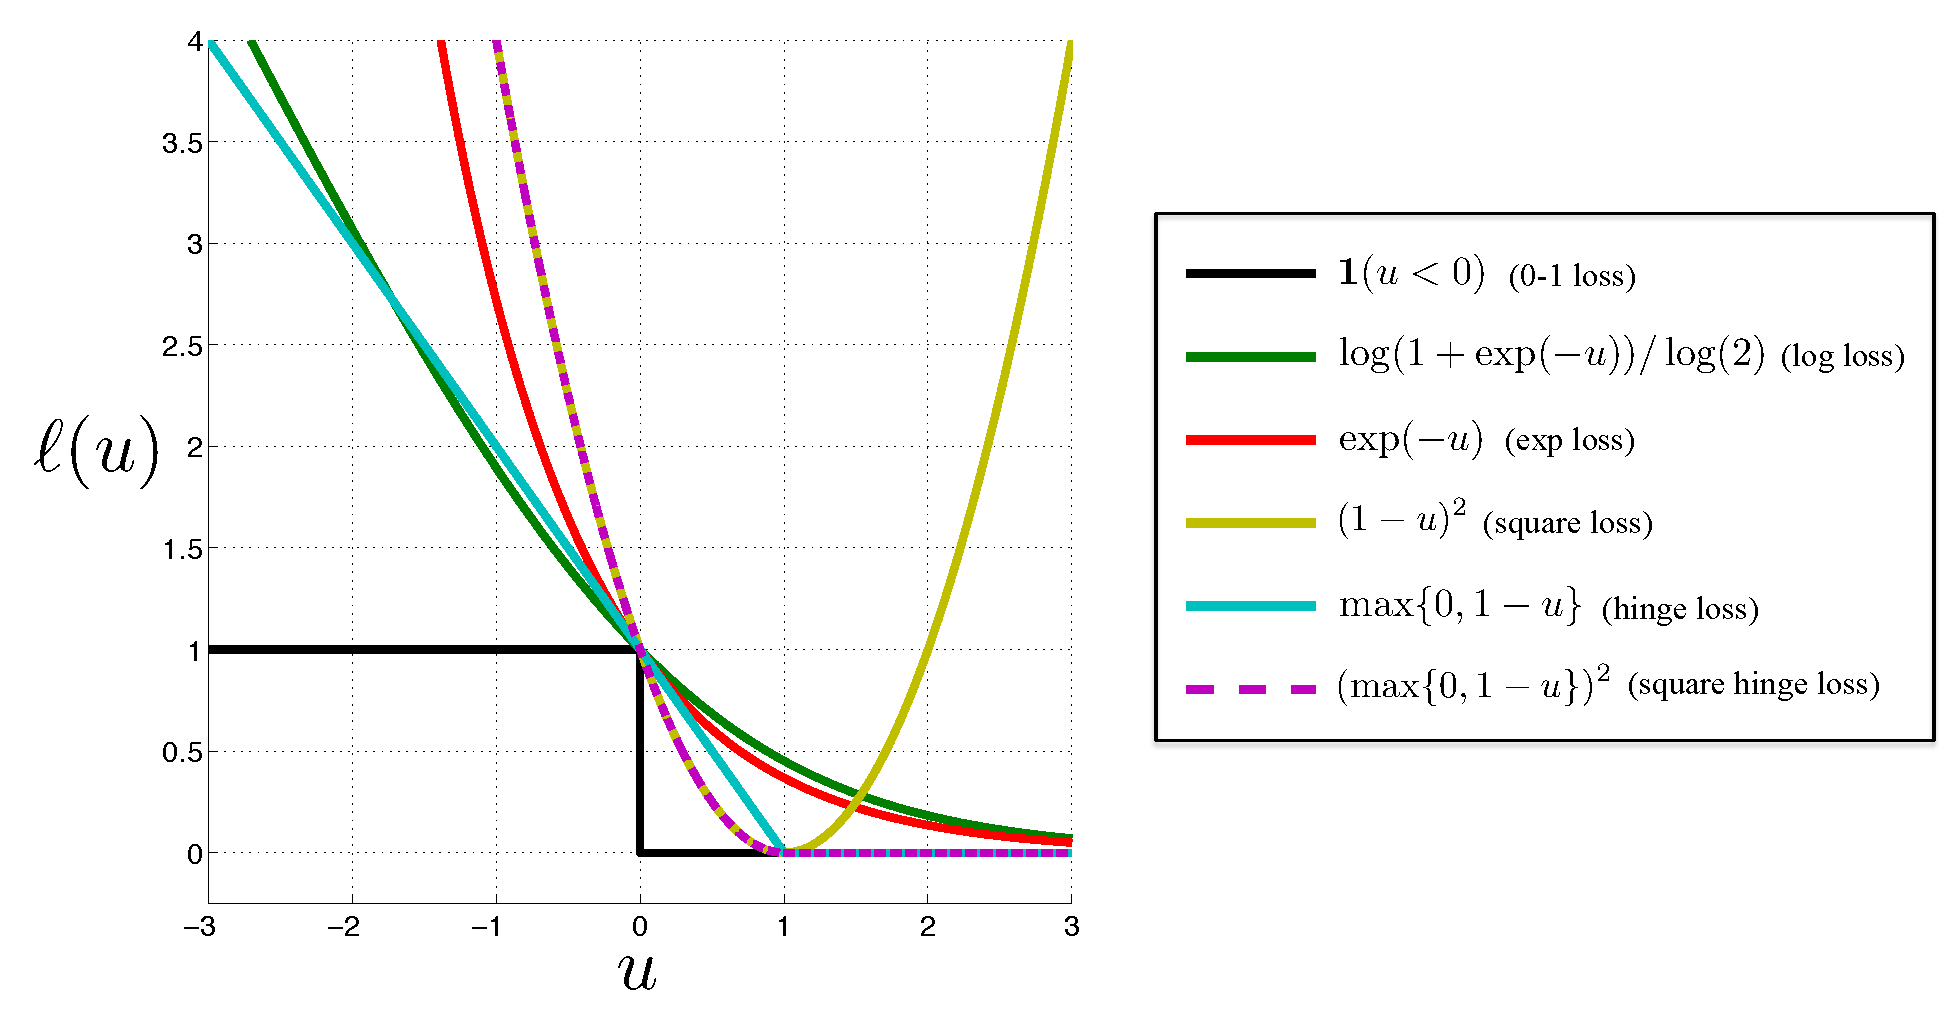
\includegraphics[width=0.99\textwidth]{figs/losses.pdf}
\caption[Convex surrogate supervised loss functions.]{Convex surrogate supervised loss functions.}
\label{fig:surrogates}
\end{center}
\end{figure}

Using a linear representation, we have the following optimization problem to learn our model from training data:
\begin{align}
&\minimize_\w \cL_{0/1}(h,S) = \\ &\minimize_\w \frac{1}{m}\sum_{j=1}^m 
\Ind\left( \argmax_y [\w \cdot \f(x^{(j)},y)] \neq y^{(j)}\right)
\end{align}
The above optimization is extremely difficult to solve in high dimensions 
because it is non-convex and discontinuous, leading to many poor local minima.  
In light of this, we introduce a {\em convex surrogate} to the indicator loss 
function $\ell(\cdot)$ to replace $\Ind(\cdot)$ with an upper-bound 
\citep{bishop-book}:
\begin{align}
&\minimize_\w \cL_{\ell}(h,S) = \\ &\minimize_\w \frac{1}{m}\sum_{j=1}^m 
\ell\left( \max_y \w \cdot \f(x^{(j)},y), y^{(j)}\right)
\label{eq:convex-loss}
\end{align}
There are many common choices for $\ell(\cdot)$, shown in \figref{surrogates}, 
leading to many different structured and non-structured machine learning 
algorithms.  We choose to use the {\em hinge loss} for most of this work, which 
leads to a simple and intuitive stochastic optimization algorithm.  The hinge 
loss is of the form $\ell(u) = \max (0,1-u) \defn [1-u]_+$, giving us the 
following optimization problem:
\begin{align}
\minimize_\w \frac{1}{m}\sum_{j=1}^m \left[ \max_y \w \cdot \f(x^{(j)},y) - \w 
\cdot \f(x,y^{(j)}) + 1\right]_+
\label{eq:svm-noreg}
\end{align}
Depending on the training set, this form of learning function may have issues.  
Particularly, if the training set is {\em separable}, there are many possible 
$\w$'s that will achieve an optimum value of $0$ in \equref{svm-noreg}. For 
example, if a $\w$ is a minimizer, so is $10\cdot \w$.  Thus, we add an 
additional regularization term that seeks to find a low error $\w$, as well as 
a simple $\w$---one whose weights are small. To this effect, a regularized form 
is
\begin{align}
\minimize_\w \frac{\lambda}{2}||\w||_2^2 + \frac{1}{m}\sum_{j=1}^m \left[ 
\max_y \w \cdot \f(x^{(j)},y) - \w \cdot \f(x,y^{(j)}) + 1\right]_+
\label{eq:svm}
\end{align}
 which encourages $\w$ to be small in an $L_2$-norm sense.  The meta-parameter 
$\lambda$ balances how much we care about model simplicity (first term) versus 
training accuracy (second term).  Model simplicity implies a better chance of 
generalizing to new data, at the risk of being too restrained to learn an 
effective classifier.  Such concerns about model underfitting or overfitting 
and the tradeoff between model bias and model variance are well-studied in the 
machine learning literature, especially for linear classifiers. See 
\citet{bishop-book, esl-book} for rigorous treatments.

\subsection{Learning algorithms}\label{sec:learning-algs}

Any convex learning function of the form of \equref{convex-loss} lends itself 
to a variety of optimization algorithms.  Because we are guaranteed to reach a 
global optimum (modulo numerical precision and computational limitations), we 
focus on choosing a method that is quick and simple.  Stochastic first-order 
descent methods estimate the gradient of the function one data point at a time, 
and are attractive due to their low memory requirements and fast convergence 
rates per example examined~\citep{shalev07}.

Using \equref{svm}, the second term is piecewise-linear, and we take stochastic 
subgradient steps to optimize it, also known as structured 
perceptron~\citep{Collins2002}. Given a single supervised example $(x,y)$, we 
make the following update if the second, hinge loss term of~\equref{svm} (\ie, 
the subgradient) is non-zero:
\begin{align}
\w' \leftarrow (1-\eta\lambda)\w + \eta \left( \f(x,y) - \f(x,y^\star) \right).
\end{align}
where, again, $y^\star = \argmax_y' \w \cdot \f(x,y')$.
